\documentclass[a4paper,12pt]{article}
\usepackage{indentfirst}
\usepackage[latin1,utf8]{inputenc}
\usepackage[portuges]{babel}
\usepackage[a4paper,portrait]{geometry}
\usepackage{amsmath} 
\usepackage{multicol}
\usepackage{makeidx} 
\usepackage{color} 
\usepackage{fancyhdr}
\usepackage{url}
\usepackage{lipsum}
\usepackage[pdftex]{graphicx}
\usepackage{epstopdf}
\usepackage{graphics}
\usepackage{fancyhdr}
\usepackage{cleveref}
\usepackage{hyperref}
\usepackage{fixltx2e}
\usepackage{tabularx, booktabs}
\usepackage[utf8]{inputenc}
\usepackage{geometry}
\usepackage{xlop}

\input epsf

\makeindex

\begin{document}
\renewcommand{\sfdefault}{lmss}
\renewcommand{\familydefault}{\sfdefault}
\fontfamily{lmss}\selectfont

\title{\bf Relatório de Sistemas Digitais \\
Traballho L2\\
Circuitos Combinatórios Típicos}
\author{João Oliveira\\
Tomás A. Reis\\
\\
Instituto Superior Técnico \\
Universidade de Lisboa}
\date{10 de Abril de 2014 \\
Quinta-Feira LSD1}
\maketitle

\pagebreak
\section{Introdução}
Neste trabalho tem-se como objectivo a concepção e montagem de um circuito 
capaz de seleccionar uma função que depende de um {\it input} A no intervalo 
[0;15], e uma saída para este sinal. Para executar esta selecção é também 
dado um {\it input} I no intervalo [0;7] em que o digito mais significativo 
selecciona a função e os outros dois a saída. 
\par
Neste relatório apresentamos uma concretização possível deste circuito 
utilizando o mínimo material, partindo do disponível no laboratório. Inclui, 
igualmente, uma explicação do funcionamento das várias funções lógicas e 
a forma como estão ligadas de forma a realizar as funções pretendidas, bem 
como a listagem dos circuitos integrados necessários à sua montagem.
\par
Também são apresentados os resultados verificados em laboratório após a 
montagem do circuito como apresentado.

\section{Projecto}
\subsection{Cálculo das Constantes}
O número de aluno utilizado foi o 78811, visto ser o de menor valor. Como 
podemos observar nas divisões apresentadas em seguida, os restos da primeira e 
segunda divisão inteira por oito, que correspondem aos dois dígitos menos 
significativos em base oito, são idênticos e de valor 3. 
\par
\vspace*{1\baselineskip}
\hspace{20pt} \opdiv[maxdivstep=4]{78811}{8} \hspace{60pt} 
\opdiv[maxdivstep=4]{9851}{8}
\vspace*{1\baselineskip}
\par
Assim, teremos:
\begin{equation}
K_1=K_0=3
\end{equation}
\subsection{Diagrama Lógico}
\subsubsection{O Circuito}
O objectivo é construir um circuito que recebe um um número A no intervalo 
[0;15], representado pelos dígitos binários a\textsubscript{3}, 
a\textsubscript{2}, a\textsubscript{1} e a\textsubscript{0} (sendo 
a\textsubscript{3} o {\it bit} mais significativo e a\textsubscript{0} o menos) 
e três {\it bits} de selecção I\textsubscript{2}, I\textsubscript{1} e 
I\textsubscript{0}, seleccionando uma de duas funções de A, e uma de quatro 
saídas, representadas por S\textsubscript{3}, S\textsubscript{2}, 
S\textsubscript{1} e S\textsubscript{0}, para esta função. A função 
f\textsubscript{1} é ``1'' excepto quando A = K\textsubscript{1}, enquanto 
f\textsubscript{0} é ``1'' apenas quando A = K\textsubscript{0}. A 
função é seleccionada pelo {\it bit} I\textsubscript{2} e a saída pelos 
{\it bits} I\textsubscript{1} e I\textsubscript{0}, correspondendo cada 
combinação destes dois {\it bits} à saída cujo número de identificação 
é representado em binário por I\textsubscript{1}I\textsubscript{0}.
\par
\subsubsection{Funções a Seleccionar}
As duas funções a seleccionar dependem do valor de A, sendo que a primeira função f\textsubscript{1} tem valor ``0'' apenas quando A igual a uma constante K\textsubscript{1}, enquanto f\textsubscript{0} é 1 apenas quando A é igual a uma constante K\textsubscript{0}.
\par
De forma a realizarmos estas funções concluímos que o mais simples seria 
utilizarmos um {\it decoder} 3:8. Este circuito recebe três {\it bits} de 
selecção e três para o {\it enable} e tem oito saídas, numeradas de 0 a 7. 
Quando o {\it enable} tem valor 3 (estando duas entradas negadas isto 
corresponde a ``1'' na entrada positiva e ``0'' nas entradas negativas), a 
saída cujo número corresponde ao número codificado nos {\it bits} de 
selecção fica activa. Nos {\it decoders} usados, que têm as saídas negadas, 
isto corresponde a ter a saída seleccionada em {\it ``low''} e as restantes em 
{\it ``high''}. Caso o {\it enable} não seja igual a 3, todas as saídas 
estão inactivas em  {\it ``high''}.
\par
Como as constantes são inferiores a 8, ligamos a\textsubscript{3} às duas 
entradas negadas do {\it enable}. Assim, como A é certamente diferente de K 
quando a\textsubscript{3} tem valor ``1'', o {\it decoder} fica inactivo nesta 
situação. A entrada positiva do enable é ligada ao VCC de forma a estar 
sempre no valor ``1''. 
\par
Os restantes dígitos de A são ligados às entradas do {\it decoder} para que, 
quando a\textsubscript{3} tem valor ``0'', a saída seleccionada corresponda ao 
valor de A. Como f\textsubscript{1} tem valor ``1''  sempre que A é distinto 
de K\textsubscript{1} ligamos esta função à saída do {\it decoder} de 
número K\textsubscript{1}, que está negada. Analogamente ligamos 
f\textsubscript{0} à saída K\textsubscript{0} com uma porta NOT.
\par
Neste caso, como ambas as constantes são 3, isto corresponde a ligar 
f\textsubscript{1} directamente à saída 3 deste {\it decoder} e 
f\textsubscript{0} a uma porta NOT ligada a esta mesma saída. Estas funções 
poderiam também ser concretizadas com portas lógicas, como portas NAND ou 
NOR, porém tal não levaria nem a um menor número de circuitos integrados 
utilizados nem a uma simplificação da montagem.
\par

\begin{figure}
\centering
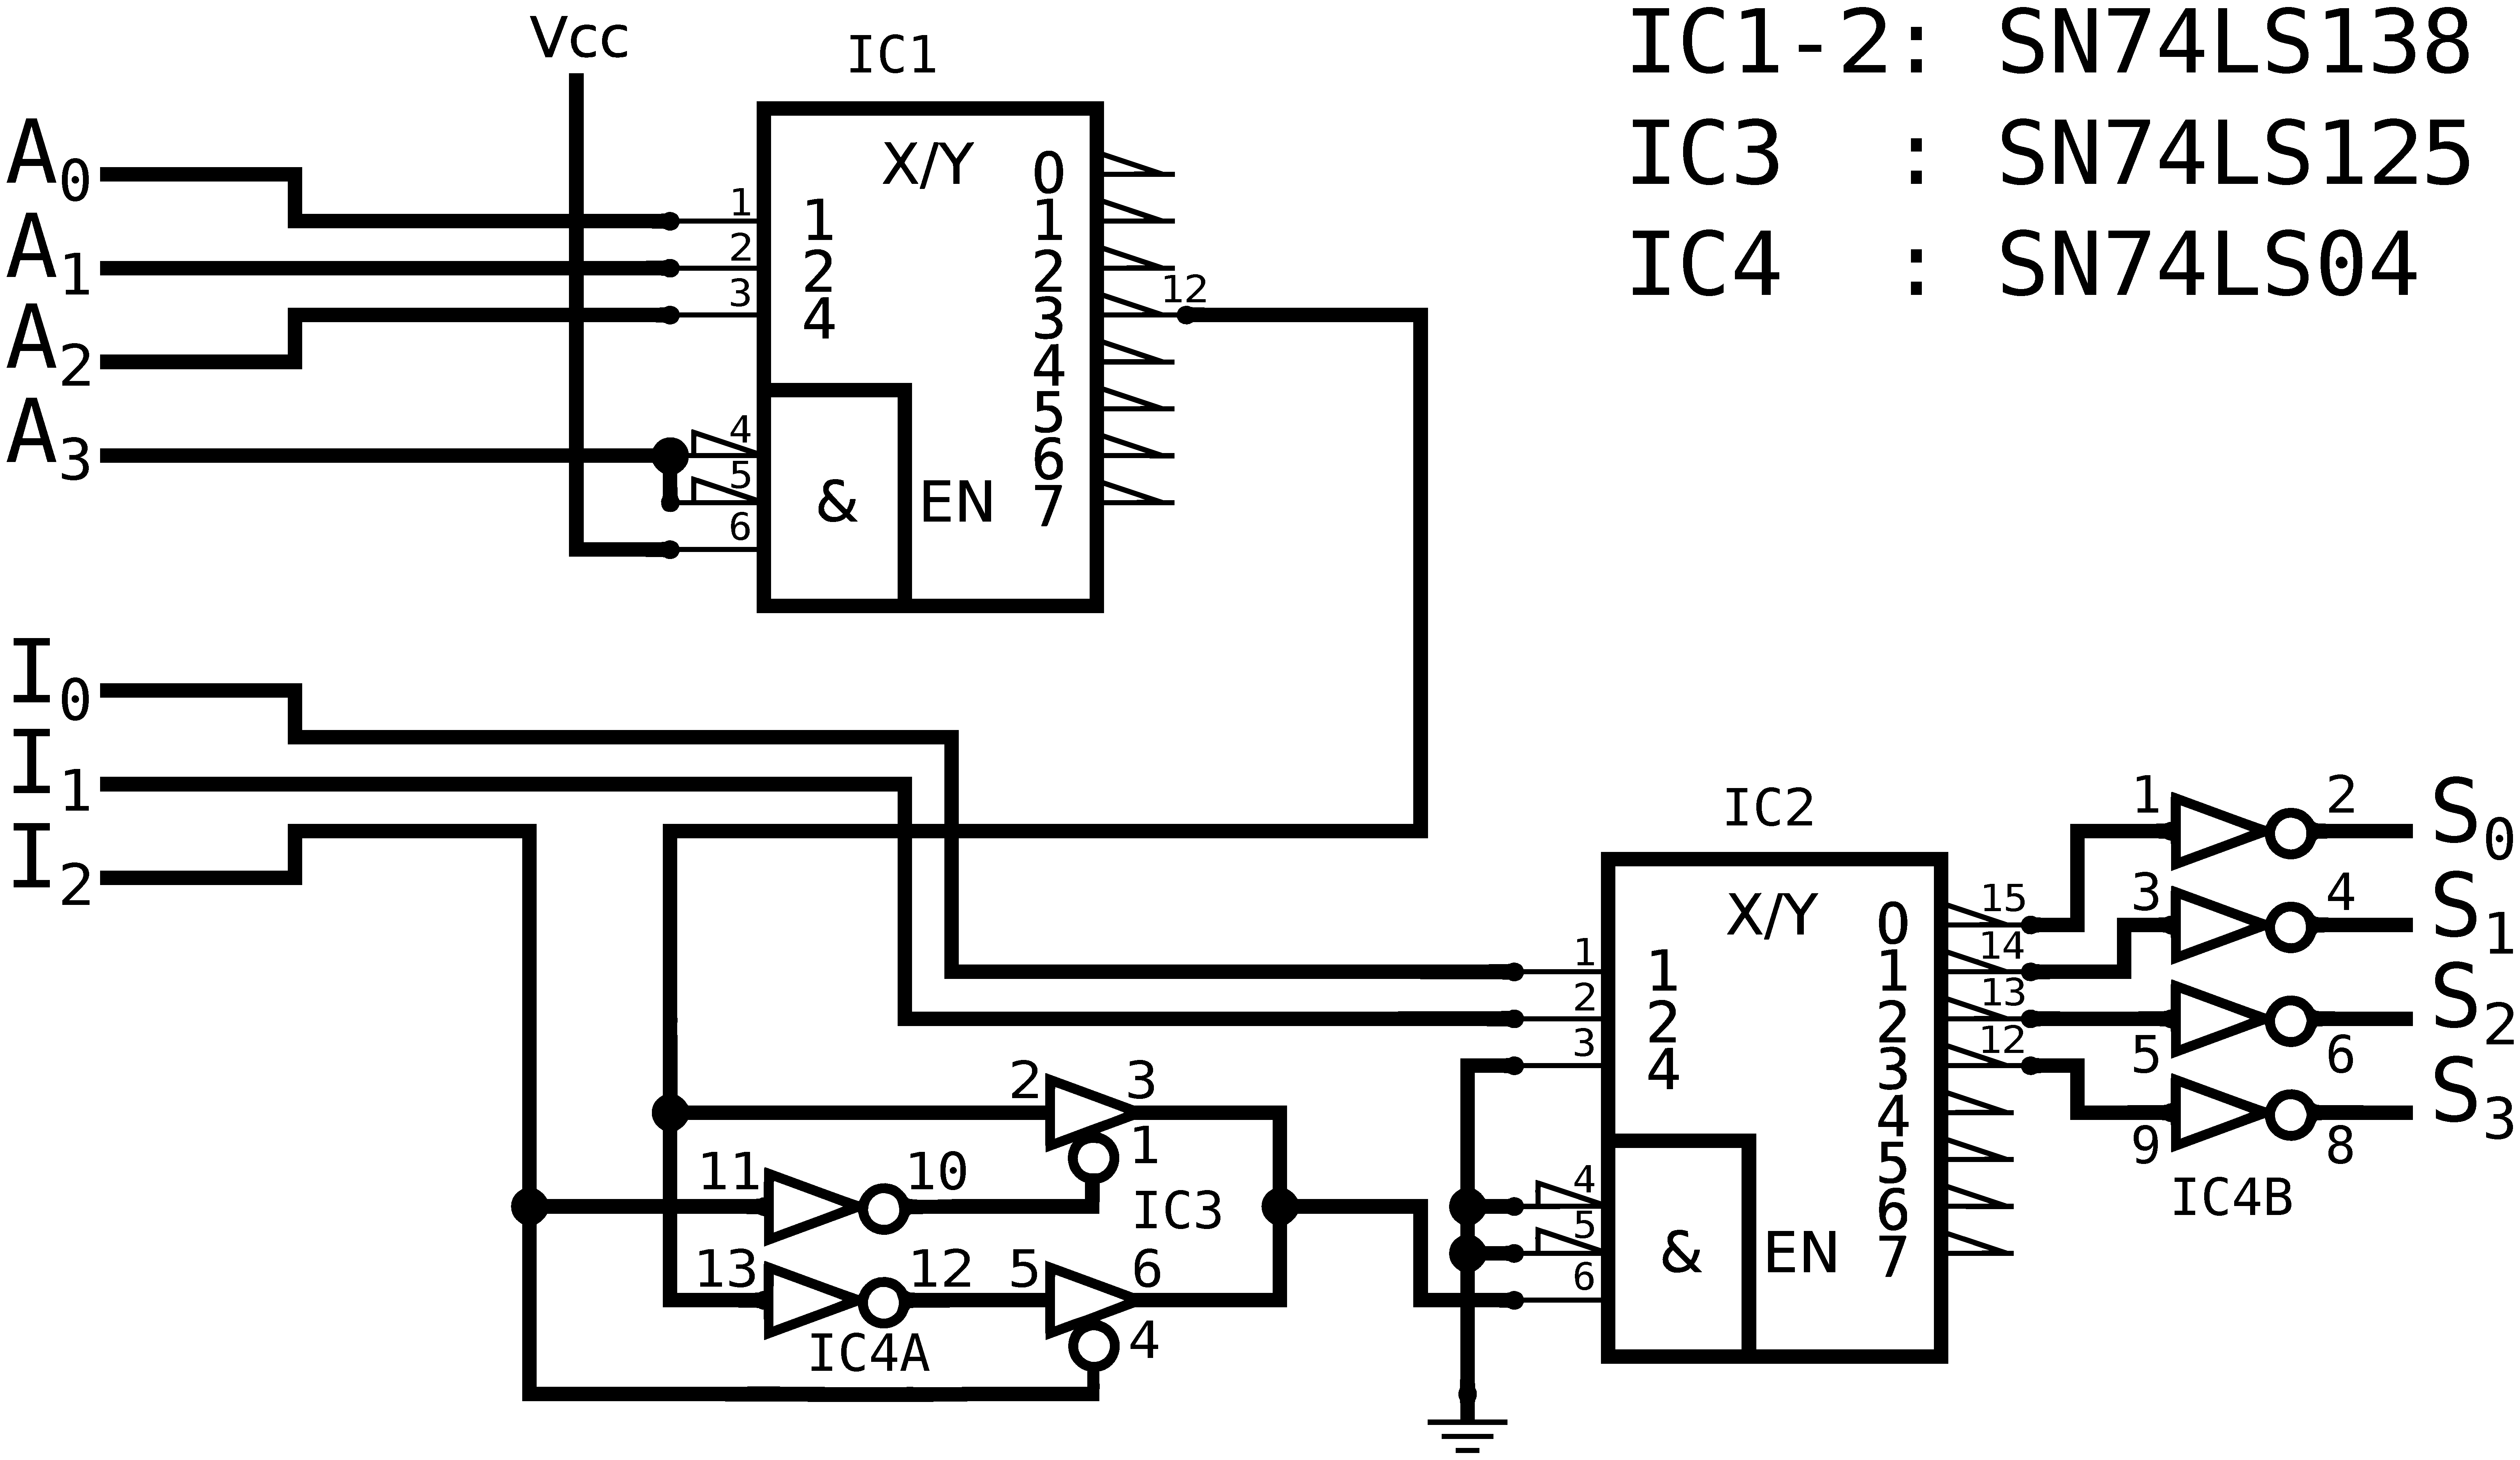
\includegraphics[scale=.1]{logigrama.eps}
\caption{Diagrama Lógico}
\end{figure}

\subsubsection{Selecção da Função}
Para a selecção das funções com o dígito I\textsubscript{2} basta dois 
{\it buffers tri-state} e uma porta NOT. Os {\it buffers tri-state} recebem um 
bit na entrada {\it ``In''} e outro na entrada {\it ``Ctrl''}. Nos {\it 
buffers} disponíveis no laboratório, que têm o {\it ``Ctrl''} negado, a 
saída {\it ``Out''} terá o valor de {\it ``In''} quando {\it ``Ctrl''} é 
``0' e estará desligada caso contrário.
\par
Num dos {\it buffers} ligamos f\textsubscript{0} à entrada {\it ``In''} e 
I\textsubscript{2} à entrada {\it ``Ctrl''}. No segundo {\it buffer} ligamos 
f\textsubscript{1} a {\it ``In''} e I\textsubscript{2} a uma porta NOT ligada 
à entrada {\it ``Ctrl''}. 
As saídas são unidas num único canal. 
\par
Desta forma, apenas um único {\it buffer} estará ligado, sendo o valor de 
f\textsubscript{1} transmitido quando I\textsubscript{2} tem valor ``1'' e 
f\textsubscript{0} caso contrário. Esta parte do circuito também poderia ter 
sido realizada com portas NAND, mas tal requereria maior complexidade de 
montagem.
\par

\subsubsection{Selecção de Saída}
Por fim, a selecção de saída é a tarefa típica de uma {\it demultiplexer} 
e como tal utilizaremos outro {\it decoder} com {\it enable}, circuito 
equivalente. Este {\it decoder} é idêntico ao {\it decoder} 3:8 descrito 
anteriormente para as funções a seleccionar.
\par 
Os {\it bits} I\textsubscript{1} e I\textsubscript{0} são ligados às entradas 
de selecção do {\it decoder} de valor menos significativo e a entrada mais 
significativa ao GND. Transformamos, efectivamente, o {\it decoder} 3:8 num 
{\it decoder} 2:4, visto que apenas as quatro primeiras saídas (ligadas a 
S\textsubscript{3}, S\textsubscript{2}, S\textsubscript{1} e 
S\textsubscript{0}) poderão ser seleccionadas consoante o valor dos dois {\it 
bits} de seleccção, I\textsubscript{1} e I\textsubscript{0}. Tal ocorre pois 
o {\it bit} mais significativo terá sempre valor ``0'', limitando o {\it 
input} de selecção ao intervalo [0;3]. Como os {\it decoders} disponíveis 
têm as saídas negadas, considerar-se-á, para efeitos de simplificação, que 
as saídas inactivas estão em {\it ``high''} (o contrário podia facilmente 
ser obtido com uma porta NOT em cada saída, porém aumentaria 
desnecessariamente o número de CIs). 
\par
Assim, ligamos a saídas da selecção de funções às duas entradas negadas do {\it 
enable} (e a entrada positiva ao VCC). Desta forma, quando este sinal, que 
corresponde à função seleccionada, tiver valor ``0'', a saída escolhida 
estará em {\it ``low''}, pois o {\it enable} estará activo, e as restantes 
estarão inactivas (em {\it ``high''}). Já quando o valor da função for 
``1'', o {\it enable} é desactivado colocando a saída seleccionada (bem como 
as restantes) estará a {\it ``high''}. Tal corresponde ao pretendido. (Este 
comportamento também está expresso na Tabela 3 na secção ``Teste do 
Circuito'').
\par
Na Figura 1 está desenhado o diagrama lógico do circuito como aqui descrito.

\subsubsection{Selecção da Função Alternativo}
Para a selecção das funções com o dígito I\textsubscript{2} optámos por uma selecção com lógica simples. Uma solução alternativa com {\it buffers tri-state} seria possível e utilizaria ligeiramente menos portas lógicas, porém corria o risco de curto-circuito sem trazer vantagens substanciais, visto nem traduzir um número de circuitos integrados diferente. 
\par
A função seleccionada f\textsubscript{s} deve ter o valor de f\textsubscript{1} quando I\textsubscript{2} é ```1'' e o valor de f\textsubscript{0} quando I\textsubscript{2} é ``0''. Isto fica traduzido pela seguinte expressão algébrica:
\begin{equation}
\begin{split}
f_s(f_1,f_0,I_2) & = I_2f_1+\overline{I_2}f_0 \\
                     & = \overline{\overline{I_2f_1+\overline{I_2}f_0}}  \\
                      & = \overline{\overline{\overline{(\overline{I_2}+\overline{f_1})}+\overline{(I_2 + \overline{f_0})}}}
                      & = \overline{\overline{\overline{(\overline{I_2}+\overline{f_1})}+\overline{(I_2 + f_1})}}} \\  
\end{split}
\end{equation}
No último passo tem-se em conta o facto de, sendo as constantes iguais, f\textsubscript{0} ser a negação de f\textsubscript{1}.
Que como, apresentado, é facilmente implementado com três portas NAND-2 e uma porta NOT. Apresenta-se na Tabela 1 a tabela de verdade desta função f\textsubscript{s} para corroboração de que obtém o pretendido.
\par
\begin{table}
\centering
\begin{tabularx}{0.75\textwidth}
{|| >{\setlength\hsize{1\hsize}\centering}X 
 |   >{\setlength\hsize{0.5\hsize}\centering}X 
    >{\setlength\hsize{0.5\hsize}\centering}X 
 || >{\centering\arraybackslash}X           ||}
\hline 
\multicolumn{1}{||c |}{{\it Bit} de Selecção} &
\multicolumn{2}{  c||}{Valores das Funções} &
\multicolumn{1}{  c||}{Valor da Saída} \\
  \hline
I\textsubscript{2} & f\textsubscript{1} & 
f\textsubscript{o} & f\textsubscript{s} \\ \hline
0  & 0  & 0  & 0\\ \hline
0  & 0  & 1  & 1\\ \hline
0  & 1  & 0  & 0\\ \hline
0  & 1  & 1  & 1\\ \hline
1  & 0  & 0  & 0\\ \hline
1  & 0  & 1  & 0\\ \hline
1  & 1  & 0  & 1\\ \hline
1  & 1  & 1  & 1\\ \hline

\end{tabularx}
\caption{Tabela da Função de Selecção}
\end{table}

\subsubsection{Selecção de Saída}
Por fim, a selecção de saída é a tarefa típica de uma {\it demultiplexer} 
e como tal utilizaremos outro {\it decoder} com {\it enable}, circuito 
equivalente. Este {\it decoder} é idêntico ao {\it decoder} 3:8 descrito 
anteriormente para as funções a seleccionar.
\par 
Os {\it bits} I\textsubscript{1} e I\textsubscript{0} são ligados às entradas 
de selecção do {\it decoder} de valor menos significativo e a entrada mais 
significativa ao GND. Transformamos, efectivamente, o {\it decoder} 3:8 num 
{\it decoder} 2:4, visto que apenas as quatro primeiras saídas (ligadas a 
S\textsubscript{3}, S\textsubscript{2}, S\textsubscript{1} e 
S\textsubscript{0}) poderão ser seleccionadas consoante o valor dos dois {\it 
bits} de seleccção, I\textsubscript{1} e I\textsubscript{0}. Tal ocorre pois 
o {\it bit} mais significativo terá sempre valor ``0'', limitando o {\it 
input} de selecção ao intervalo [0;3]. Como os {\it decoders} disponíveis 
têm as saídas negadas, considerar-se-á, para efeitos de simplificação, que 
as saídas inactivas estão em {\it ``high''} (o contrário podia facilmente 
ser obtido com uma porta NOT em cada saída, porém aumentaria 
desnecessariamente o número de CIs). 
\par
Assim, ligamos a saídas da selecção de funções às duas entradas negadas do {\it 
enable} (e a entrada positiva ao VCC). Desta forma, quando este sinal, que 
corresponde à função seleccionada, tiver valor ``0'', a saída escolhida 
estará em {\it ``low''}, pois o {\it enable} estará activo, e as restantes 
estarão inactivas (em {\it ``high''}). Já quando o valor da função for 
``1'', o {\it enable} é desactivado colocando a saída seleccionada (bem como 
as restantes) estará a {\it ``high''}. Tal corresponde ao pretendido. (Este 
comportamento também está expresso na Tabela 3 na secção ``Teste do 
Circuito'').
\par
Na Figura 1 está desenhado o diagrama lógico do circuito como aqui descrito.

\subsection{Esquema elétrico}

\begin{figure}
\centering
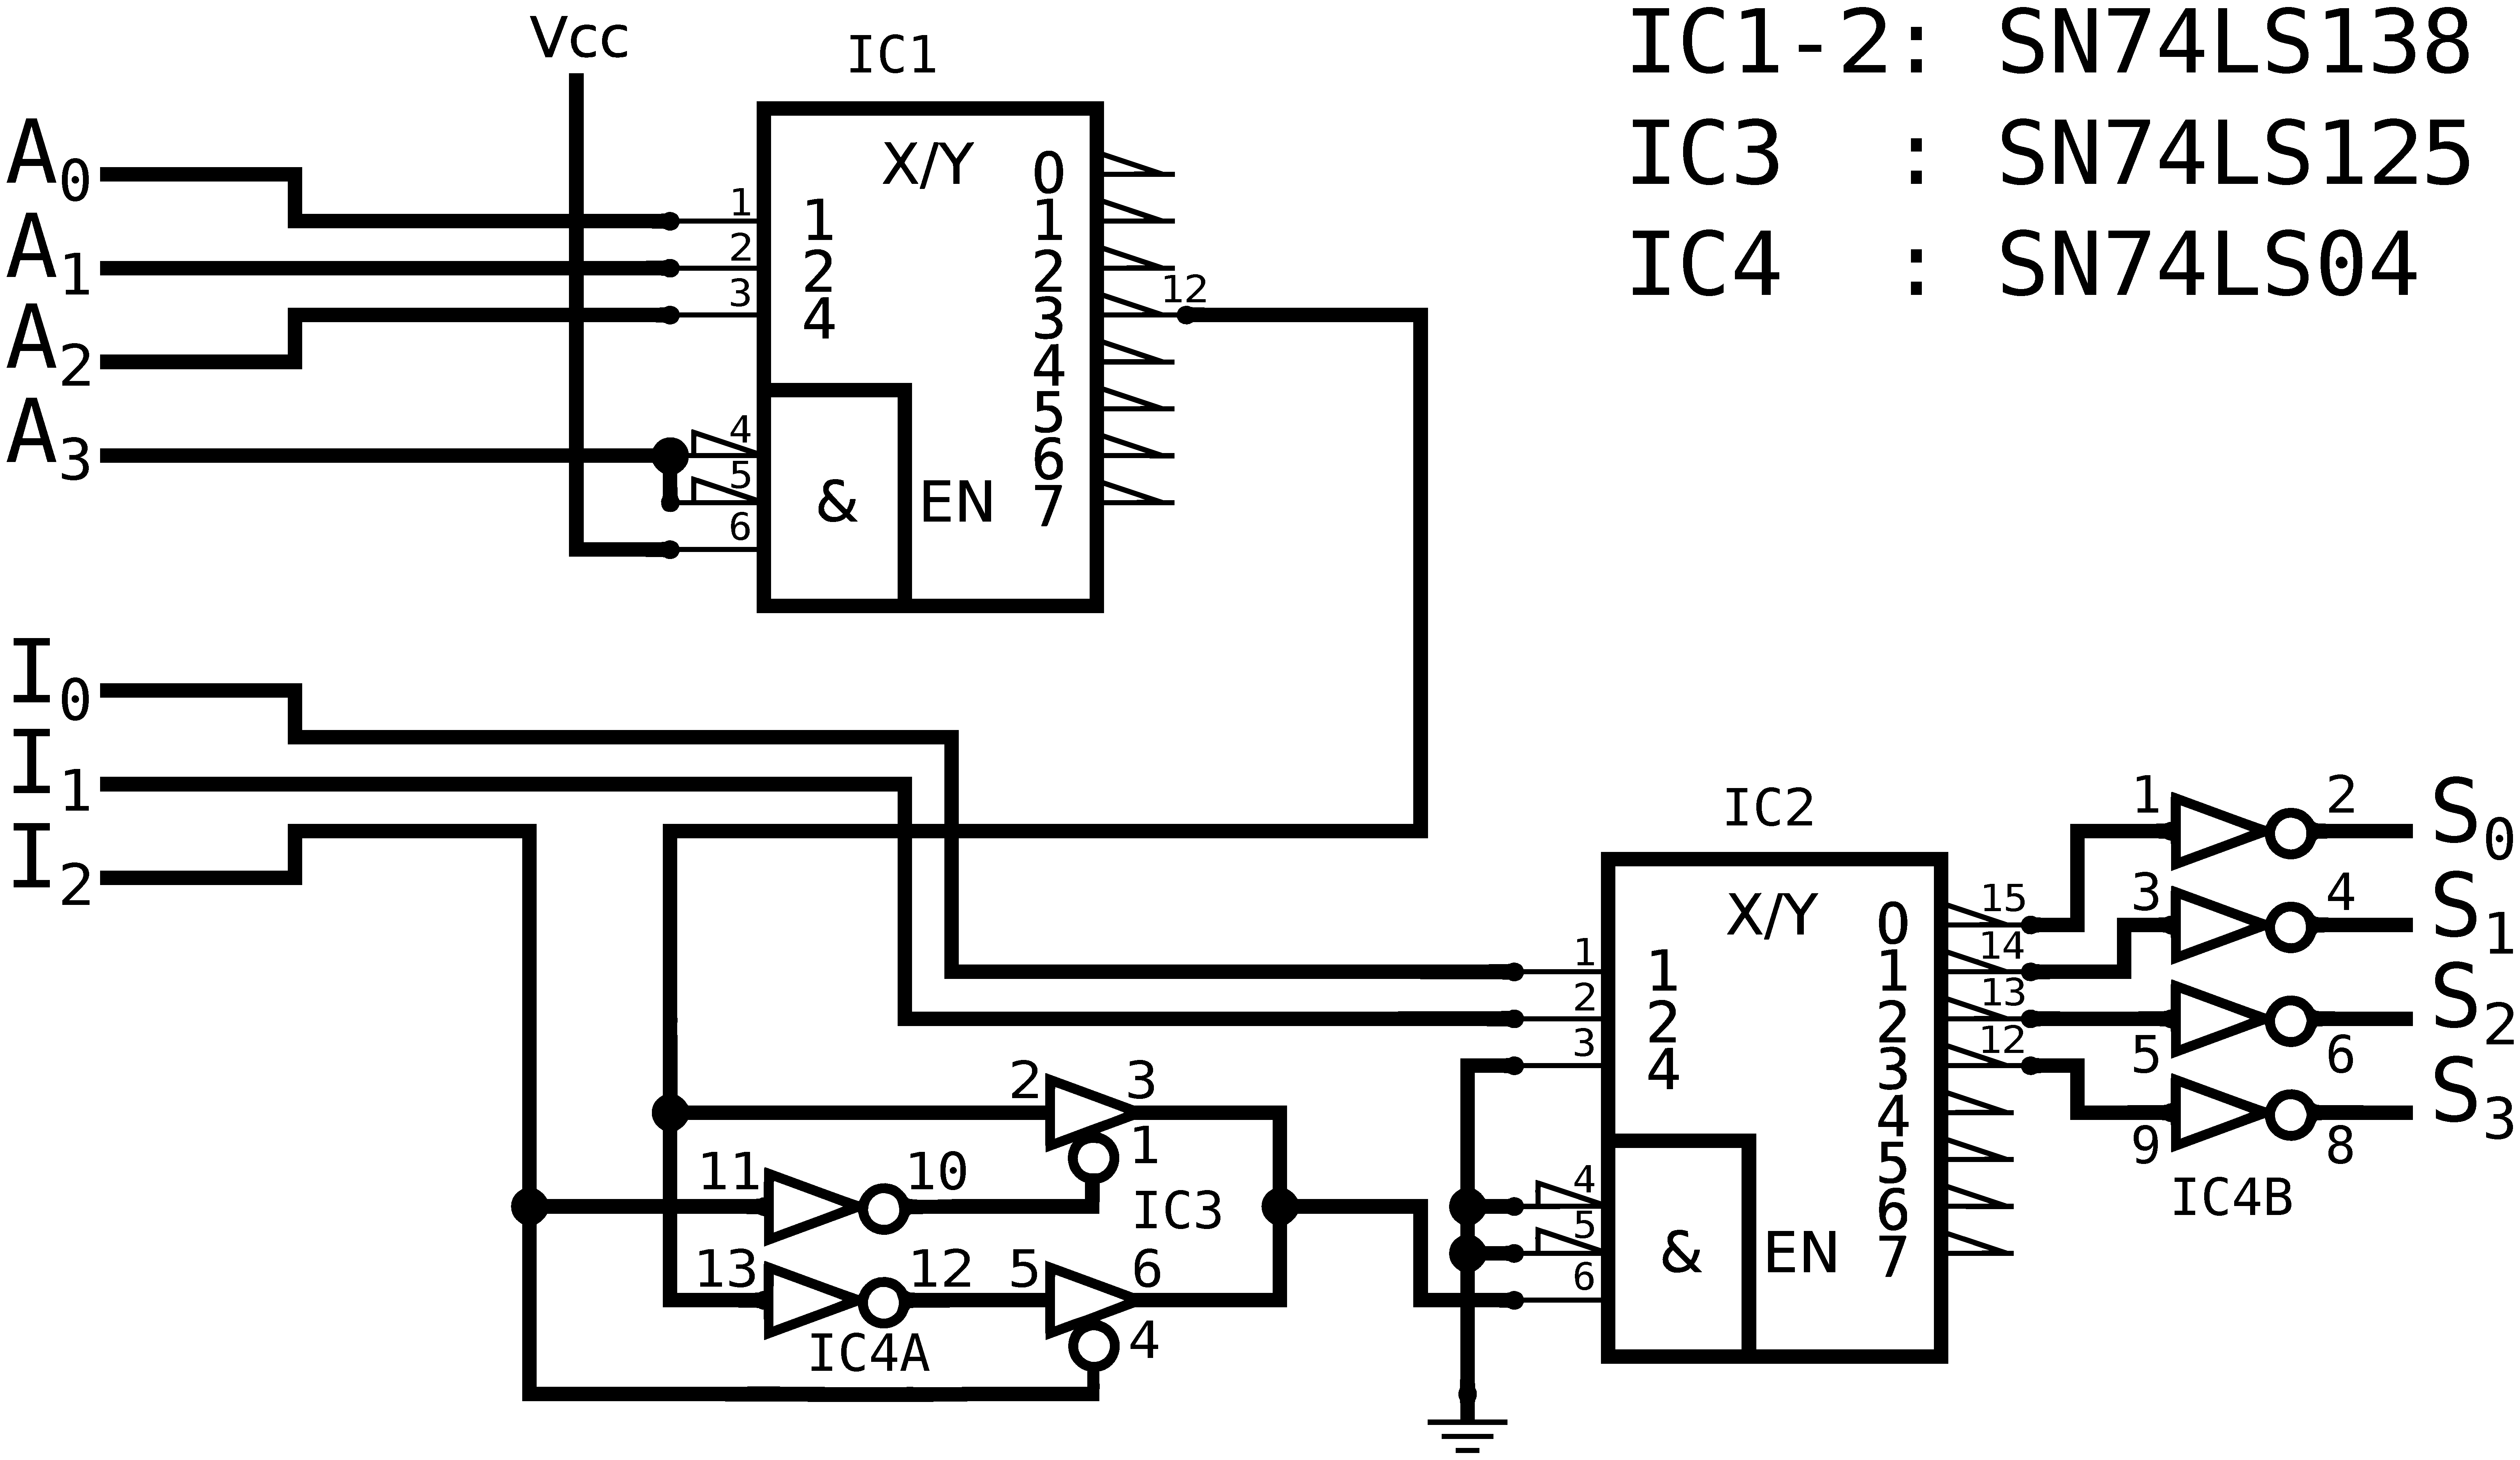
\includegraphics[scale=.1]{esqelect.eps}
\caption{Esquema Eléctrico}
\end{figure}
\par

De forma a concretizarmos o circuito, serão necessários os seguintes 
circuitos integrados:
\begin{enumerate}
    \item 2x SN74LS138 ({\it Decoders} 3:8)
    \item 1x SN74LS125!!!(Portas NAND-2)
    \item 1x SN74LS04  (Portas NOT)
\end{enumerate}
\par
As ligações deste circuito com estes componentes estão descritas no esquema 
eléctrico apresentado na Figura 2.
\section{Montagem e Teste}
\subsection{Montagem}
Montou-se o circuito na {\it breadboard} utilizando os circuitos requisitados.

\pagebreak
\subsection{Teste do circuito}
\begin{table}
\centering
\begin{tabularx}{1.0\textwidth}
{|| >{\setlength\hsize{1\hsize}\centering}X 
    >{\setlength\hsize{1\hsize}\centering}X 
    >{\setlength\hsize{1\hsize}\centering}X 
    >{\setlength\hsize{1\hsize}\centering}X 
 || >{\setlength\hsize{1\hsize}\centering}X 
    >{\setlength\hsize{1\hsize}\centering}X 
 || >{\setlength\hsize{1\hsize}\centering}X  
 |  >{\centering\arraybackslash}X           ||}
\hline 
\multicolumn{4}{||c||}{Valores de entrada} &
\multicolumn{2}{  c||}{Valores Esperados}    &
\multicolumn{2}{  c||}{Valores Obtidos} \\
  \hline
a\textsubscript{3} & a\textsubscript{2} & 
a\textsubscript{1} & a\textsubscript{0} & 
f\textsubscript{1} & f\textsubscript{0} & 
f\textsubscript{1} & f\textsubscript{0} \\ \hline
0  & 0  & 0  & 0  & L  & H  && \\ \hline
0  & 0  & 0  & 1  & L  & H  &&\\ \hline
0  & 0  & 1  & 0  & L  & H  &&\\ \hline
0  & 0  & 1  & 1  & H  & L  &&\\ \hline
0  & 1  & 0  & 0  & L  & H  &&\\ \hline
0  & 1  & 0  & 1  & L  & H  &&\\ \hline
0  & 1  & 1  & 0  & L  & H  &&\\ \hline
0  & 1  & 1  & 1  & L  & H  &&\\ \hline
1  & 0  & 0  & 0  & L  & H  &&\\ \hline
1  & 0  & 0  & 1  & L  & H  &&\\ \hline
1  & 0  & 1  & 0  & L  & H  &&\\ \hline
1  & 0  & 1  & 1  & L  & H  &&\\ \hline
1  & 1  & 0  & 0  & L  & H  &&\\ \hline
1  & 1  & 0  & 1  & L  & H  &&\\ \hline
1  & 1  & 1  & 0  & L  & H  &&\\ \hline
1  & 1  & 1  & 1  & L  & H  &&\\ \hline
\end{tabularx}
\caption{Tabela de Testes das Funções}
\end{table}

\begin{table}
\centering
\begin{tabularx}{1.0\textwidth}
{|| >{\setlength\hsize{1\hsize}\centering}X 
    >{\setlength\hsize{1\hsize}\centering}X 
    >{\setlength\hsize{1\hsize}\centering}X 
    >{\setlength\hsize{1\hsize}\centering}X 
    >{\setlength\hsize{1\hsize}\centering}X 
 || >{\setlength\hsize{1\hsize}\centering}X 
 	>{\setlength\hsize{1\hsize}\centering}X 
 	>{\setlength\hsize{1\hsize}\centering}X 
 	>{\setlength\hsize{1\hsize}\centering}X 
 || >{\centering\arraybackslash}X  
 |  >{\centering\arraybackslash}X 
 |  >{\setlength\hsize{1\hsize}\centering}X 
 |  >{\centering\arraybackslash}X ||}
\hline 
\multicolumn{5}{||c||}{Valores de entrada} & 
\multicolumn{4}{  c||}{Valores Esperados} & 
\multicolumn{4}{  c||}{Valores Obtidos} \\
\hline

I\textsubscript{2} & I\textsubscript{1} & 
I\textsubscript{0} & 
f\textsubscript{1} & f\textsubscript{0} & 
S\textsubscript{3} & S\textsubscript{2} & 
S\textsubscript{1} & S\textsubscript{0} &
S\textsubscript{3} & S\textsubscript{2} & 
S\textsubscript{1} & S\textsubscript{0} 
\\ \hline
0  & 0  & 0  & X  & 0  & H  & H  & H  & L  &&&& \\ \hline
0  & 0  & 0  & X  & 1  & H  & H  & H  & H  &&&&\\ \hline
0  & 0  & 1  & X  & 0  & H  & H  & L  & H  &&&&\\ \hline
0  & 0  & 1  & X  & 1  & H  & H  & H  & H  &&&&\\ \hline
0  & 1  & 0  & X  & 0  & H  & L  & H  & H  &&&&\\ \hline
0  & 1  & 0  & X  & 1  & H  & H  & H  & H  &&&&\\ \hline
0  & 1  & 1  & X  & 0  & L  & H  & H  & H  &&&&\\ \hline
0  & 1  & 1  & X  & 1  & H  & H  & H  & H  &&&&\\ \hline
1  & 0  & 0  & 0  & X  & H  & H  & H  & L  &&&&\\ \hline
1  & 0  & 0  & 1  & X  & H  & H  & H  & H  &&&&\\ \hline
1  & 0  & 1  & 0  & X  & H  & H  & L  & H  &&&&\\ \hline
1  & 0  & 1  & 1  & X  & H  & H  & H  & H  &&&&\\ \hline
1  & 1  & 0  & 0  & X  & H  & L  & H  & H  &&&&\\ \hline
1  & 1  & 0  & 1  & X  & H  & H  & H  & H  &&&&\\ \hline
1  & 1  & 1  & 0  & X  & L  & H  & H  & H  &&&&\\ \hline
1  & 1  & 1  & 1  & X  & H  & H  & H  & H  &&&&\\ \hline
\end{tabularx}
\caption{Tabela de Teste das Saídas}
\end{table}
\pagebreak

\section{Conclusão}
Neste trabalho concebeu-se e montou-se uma unidade combinatória capaz de executar duas funções de um número A, seleccionar uma destas e apresentá-la numa saída seleccionada entre quatro. Para tal, encontrou-se um equilíbrio de utilização de circuitos integrados utilizando tanto funções mais complexas, como os {\it decoders}, e portas lógicas mais simples, como as portas NAND-2 e NOT. Verificou-se que uma solução com a utilização de dois {\it decoders}, um para obter as funções e outro para seleccionar as saídas, e de três portas NAND-2 para a selecção da função, bem como portas NOT adicionais, concretizava a tarefa de forma eficiente. Esta foi a solução montada em laboratório.

\end{document}

-----------> footnotes
